\documentclass[twoside]{book}

% Packages required by doxygen
\usepackage{fixltx2e}
\usepackage{calc}
\usepackage{doxygen}
\usepackage[export]{adjustbox} % also loads graphicx
\usepackage{graphicx}
\usepackage[utf8]{inputenc}
\usepackage{makeidx}
\usepackage{multicol}
\usepackage{multirow}
\PassOptionsToPackage{warn}{textcomp}
\usepackage{textcomp}
\usepackage[nointegrals]{wasysym}
\usepackage[table]{xcolor}

% Font selection
\usepackage[T1]{fontenc}
\usepackage[scaled=.90]{helvet}
\usepackage{courier}
\usepackage{amssymb}
\usepackage{sectsty}
\renewcommand{\familydefault}{\sfdefault}
\allsectionsfont{%
  \fontseries{bc}\selectfont%
  \color{darkgray}%
}
\renewcommand{\DoxyLabelFont}{%
  \fontseries{bc}\selectfont%
  \color{darkgray}%
}
\newcommand{\+}{\discretionary{\mbox{\scriptsize$\hookleftarrow$}}{}{}}

% Page & text layout
\usepackage{geometry}
\geometry{%
  a4paper,%
  top=2.5cm,%
  bottom=2.5cm,%
  left=2.5cm,%
  right=2.5cm%
}
\tolerance=750
\hfuzz=15pt
\hbadness=750
\setlength{\emergencystretch}{15pt}
\setlength{\parindent}{0cm}
\setlength{\parskip}{3ex plus 2ex minus 2ex}
\makeatletter
\renewcommand{\paragraph}{%
  \@startsection{paragraph}{4}{0ex}{-1.0ex}{1.0ex}{%
    \normalfont\normalsize\bfseries\SS@parafont%
  }%
}
\renewcommand{\subparagraph}{%
  \@startsection{subparagraph}{5}{0ex}{-1.0ex}{1.0ex}{%
    \normalfont\normalsize\bfseries\SS@subparafont%
  }%
}
\makeatother

% Headers & footers
\usepackage{fancyhdr}
\pagestyle{fancyplain}
\fancyhead[LE]{\fancyplain{}{\bfseries\thepage}}
\fancyhead[CE]{\fancyplain{}{}}
\fancyhead[RE]{\fancyplain{}{\bfseries\leftmark}}
\fancyhead[LO]{\fancyplain{}{\bfseries\rightmark}}
\fancyhead[CO]{\fancyplain{}{}}
\fancyhead[RO]{\fancyplain{}{\bfseries\thepage}}
\fancyfoot[LE]{\fancyplain{}{}}
\fancyfoot[CE]{\fancyplain{}{}}
\fancyfoot[RE]{\fancyplain{}{\bfseries\scriptsize Generated by Doxygen }}
\fancyfoot[LO]{\fancyplain{}{\bfseries\scriptsize Generated by Doxygen }}
\fancyfoot[CO]{\fancyplain{}{}}
\fancyfoot[RO]{\fancyplain{}{}}
\renewcommand{\footrulewidth}{0.4pt}
\renewcommand{\chaptermark}[1]{%
  \markboth{#1}{}%
}
\renewcommand{\sectionmark}[1]{%
  \markright{\thesection\ #1}%
}

% Indices & bibliography
\usepackage{natbib}
\usepackage[titles]{tocloft}
\setcounter{tocdepth}{3}
\setcounter{secnumdepth}{5}
\makeindex

% Hyperlinks (required, but should be loaded last)
\usepackage{ifpdf}
\ifpdf
  \usepackage[pdftex,pagebackref=true]{hyperref}
\else
  \usepackage[ps2pdf,pagebackref=true]{hyperref}
\fi
\hypersetup{%
  colorlinks=true,%
  linkcolor=blue,%
  citecolor=blue,%
  unicode%
}

% Custom commands
\newcommand{\clearemptydoublepage}{%
  \newpage{\pagestyle{empty}\cleardoublepage}%
}

\usepackage{caption}
\captionsetup{labelsep=space,justification=centering,font={bf},singlelinecheck=off,skip=4pt,position=top}

%===== C O N T E N T S =====

\begin{document}

% Titlepage & ToC
\hypersetup{pageanchor=false,
             bookmarksnumbered=true,
             pdfencoding=unicode
            }
\pagenumbering{alph}
\begin{titlepage}
\vspace*{7cm}
\begin{center}%
{\Large My Project \\[1ex]\large 0.\+5 }\\
\vspace*{1cm}
{\large Generated by Doxygen 1.8.13}\\
\end{center}
\end{titlepage}
\clearemptydoublepage
\pagenumbering{roman}
\tableofcontents
\clearemptydoublepage
\pagenumbering{arabic}
\hypersetup{pageanchor=true}

%--- Begin generated contents ---
\chapter{Todo List}
\label{todo}
\Hypertarget{todo}

\begin{DoxyRefList}
\item[\label{todo__todo000002}%
\Hypertarget{todo__todo000002}%
Member \hyperlink{classAFMatrix_a918b5f7c03cb3a305ec94e08afd3e09a}{A\+F\+Matrix$<$ T $>$\+:\+:A\+F\+Matrix} (A\+F\+Matrix$<$ T $>$ $\ast$copy\+From)]Make this effecient and non-\/copying  
\item[\label{todo__todo000003}%
\Hypertarget{todo__todo000003}%
Member \hyperlink{classAFMatrix_a0dfd54218d171d086a738a0525c5946e}{A\+F\+Matrix$<$ T $>$\+:\+:A\+F\+Matrix} (int num\+Rows, int num\+Cols, vector$<$ T $>$ $\ast$copy\+From\+Array)]Make this effecient and non-\/copying  
\item[\label{todo__todo000004}%
\Hypertarget{todo__todo000004}%
Member \hyperlink{classAFMatrix_a63cc8c6b50d757fc75049a35a9123588}{A\+F\+Matrix$<$ T $>$\+:\+:copy\+Values} (A\+F\+Matrix$<$ T $>$ $\ast$dst, vector$<$ T $>$ $\ast$src)]Clarify how things work if matrices can be row-\/major or column-\/major.  
\item[\label{todo__todo000001}%
\Hypertarget{todo__todo000001}%
Member \hyperlink{classAFMatrix_a124e51921d4275e00354d3af98399d1e}{A\+F\+Matrix$<$ T $>$\+:\+:vals} ]Is vals dynamically allocated or what?? $\vert$ a b $\vert$~\newline
$\vert$ c d $\vert$ = \mbox{[}a b c d e f\mbox{]}~\newline
$\vert$ e f $\vert$~\newline

\end{DoxyRefList}
\chapter{Hierarchical Index}
\section{Class Hierarchy}
This inheritance list is sorted roughly, but not completely, alphabetically\+:\begin{DoxyCompactList}
\item \contentsline{section}{A\+F\+Activation\+Function}{\pageref{class_a_f_activation_function}}{}
\begin{DoxyCompactList}
\item \contentsline{section}{Re\+LU}{\pageref{class_re_l_u}}{}
\end{DoxyCompactList}
\item \contentsline{section}{A\+F\+Matrix$<$ T, R\+O\+WS, C\+O\+LS $>$}{\pageref{class_a_f_matrix}}{}
\item \contentsline{section}{A\+F\+Matrix$<$ double, L\+E\+N\+\_\+\+O\+UT, L\+E\+N\+\_\+\+IN $>$}{\pageref{class_a_f_matrix}}{}
\item \contentsline{section}{Layer$<$ L\+E\+N\+\_\+\+IN, L\+E\+N\+\_\+\+O\+UT $>$}{\pageref{class_layer}}{}
\item \contentsline{section}{Net$<$ T $>$}{\pageref{class_net}}{}
\end{DoxyCompactList}

\chapter{Class Index}
\section{Class List}
Here are the classes, structs, unions and interfaces with brief descriptions\+:\begin{DoxyCompactList}
\item\contentsline{section}{\hyperlink{class_a_f_activation_function}{A\+F\+Activation\+Function$<$ T, N, M $>$} }{\pageref{class_a_f_activation_function}}{}
\item\contentsline{section}{\hyperlink{class_a_f_loss_function}{A\+F\+Loss\+Function$<$ T, N, M $>$} }{\pageref{class_a_f_loss_function}}{}
\item\contentsline{section}{\hyperlink{class_a_f_matrix}{A\+F\+Matrix$<$ T, R\+O\+W\+S, C\+O\+L\+S $>$} }{\pageref{class_a_f_matrix}}{}
\item\contentsline{section}{\hyperlink{class_a_f_square_loss_function}{A\+F\+Square\+Loss\+Function$<$ T, N, M $>$} }{\pageref{class_a_f_square_loss_function}}{}
\item\contentsline{section}{\hyperlink{class_identity_function}{Identity\+Function$<$ T, N, M $>$} }{\pageref{class_identity_function}}{}
\item\contentsline{section}{\hyperlink{class_layer}{Layer$<$ L\+E\+N\+\_\+\+I\+N, L\+E\+N\+\_\+\+O\+U\+T $>$} }{\pageref{class_layer}}{}
\item\contentsline{section}{\hyperlink{class_net}{Net$<$ T $>$} }{\pageref{class_net}}{}
\item\contentsline{section}{\hyperlink{class_re_l_u}{Re\+L\+U$<$ T, N, M $>$} }{\pageref{class_re_l_u}}{}
\end{DoxyCompactList}

\chapter{Class Documentation}
\hypertarget{classAFActivationFunction}{}\section{A\+F\+Activation\+Function$<$ T $>$ Class Template Reference}
\label{classAFActivationFunction}\index{A\+F\+Activation\+Function$<$ T $>$@{A\+F\+Activation\+Function$<$ T $>$}}
Inheritance diagram for A\+F\+Activation\+Function$<$ T $>$\+:\begin{figure}[H]
\begin{center}
\leavevmode
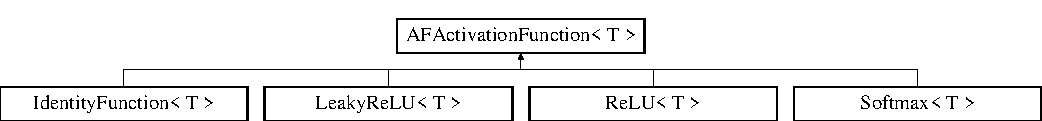
\includegraphics[height=1.618497cm]{classAFActivationFunction}
\end{center}
\end{figure}
\subsection*{Public Member Functions}
\begin{DoxyCompactItemize}
\item 
\mbox{\Hypertarget{classAFActivationFunction_afe574932347deabec0b6812ac2e9a26e}\label{classAFActivationFunction_afe574932347deabec0b6812ac2e9a26e}} 
virtual void {\bfseries evaluate} (vector$<$ T $>$ $\ast$input, vector$<$ T $>$ $\ast$output)
\item 
\mbox{\Hypertarget{classAFActivationFunction_abe287144b42493f733d2e84cd51fb03f}\label{classAFActivationFunction_abe287144b42493f733d2e84cd51fb03f}} 
virtual void {\bfseries derivative} (vector$<$ T $>$ $\ast$input, vector$<$ T $>$ $\ast$output)
\end{DoxyCompactItemize}


The documentation for this class was generated from the following file\+:\begin{DoxyCompactItemize}
\item 
src/A\+F\+Functions.\+h\end{DoxyCompactItemize}

\hypertarget{classAFLossFunction}{}\section{A\+F\+Loss\+Function$<$ T $>$ Class Template Reference}
\label{classAFLossFunction}\index{A\+F\+Loss\+Function$<$ T $>$@{A\+F\+Loss\+Function$<$ T $>$}}
Inheritance diagram for A\+F\+Loss\+Function$<$ T $>$\+:\begin{figure}[H]
\begin{center}
\leavevmode
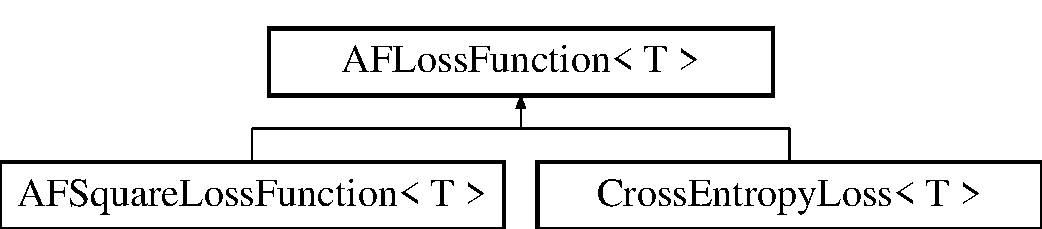
\includegraphics[height=2.000000cm]{classAFLossFunction}
\end{center}
\end{figure}
\subsection*{Public Member Functions}
\begin{DoxyCompactItemize}
\item 
\mbox{\Hypertarget{classAFLossFunction_a6c3fc3ca180b26d39275ab800b6447de}\label{classAFLossFunction_a6c3fc3ca180b26d39275ab800b6447de}} 
virtual T {\bfseries evaluate} (vector$<$ T $>$ $\ast$actual\+Vals, vector$<$ T $>$ $\ast$expected\+Vals)
\item 
\mbox{\Hypertarget{classAFLossFunction_ac04d8512f05f77d836700e02c81f3854}\label{classAFLossFunction_ac04d8512f05f77d836700e02c81f3854}} 
virtual void {\bfseries derivative} (vector$<$ T $>$ $\ast$actual\+Vals, vector$<$ T $>$ $\ast$expected\+Vals, vector$<$ T $>$ $\ast$output)
\end{DoxyCompactItemize}


The documentation for this class was generated from the following file\+:\begin{DoxyCompactItemize}
\item 
src/A\+F\+Functions.\+h\end{DoxyCompactItemize}

\hypertarget{classAFMatrix}{}\section{A\+F\+Matrix$<$ T $>$ Class Template Reference}
\label{classAFMatrix}\index{A\+F\+Matrix$<$ T $>$@{A\+F\+Matrix$<$ T $>$}}
\subsection*{Public Member Functions}
\begin{DoxyCompactItemize}
\item 
\mbox{\Hypertarget{classAFMatrix_a58a311fa4463d74220defb49a6cc43f8}\label{classAFMatrix_a58a311fa4463d74220defb49a6cc43f8}} 
{\bfseries A\+F\+Matrix} (int num\+Rows, int num\+Cols)
\item 
\hyperlink{classAFMatrix_a918b5f7c03cb3a305ec94e08afd3e09a}{A\+F\+Matrix} (\hyperlink{classAFMatrix}{A\+F\+Matrix}$<$ T $>$ $\ast$copy\+From)
\item 
\hyperlink{classAFMatrix_a0dfd54218d171d086a738a0525c5946e}{A\+F\+Matrix} (int num\+Rows, int num\+Cols, vector$<$ T $>$ $\ast$copy\+From\+Array)
\item 
int \hyperlink{classAFMatrix_a582a394221722603e21b6571e95d69a7}{get\+Index} (int row, int col)
\item 
T \hyperlink{classAFMatrix_a42f6c9d02b5507b39bf8899fea730cbf}{get\+Value} (int row, int col)
\item 
vector$<$ T $>$ $\ast$ \hyperlink{classAFMatrix_af5917b11c5f2f0ff76d9cb5f615123b5}{get\+Col} (int col)
\item 
vector$<$ T $>$ $\ast$ \hyperlink{classAFMatrix_a2474e9ce55e4a2773291304e3c48af1f}{get\+Row} (int row)
\item 
void \hyperlink{classAFMatrix_ac8a60442dd87009f6d7fe147bdce2b89}{set\+Value} (int row, int col, T new\+Value)
\item 
void \hyperlink{classAFMatrix_a2c4d9cfe683f893fd961904a788f952a}{inner\+Product} (\hyperlink{classAFMatrix}{A\+F\+Matrix}$<$ T $>$ $\ast$other, \hyperlink{classAFMatrix}{A\+F\+Matrix}$<$ T $>$ $\ast$out)
\item 
void \hyperlink{classAFMatrix_aef663e647574c6f759bee01f9c017a62}{inner\+Product} (\hyperlink{classAFMatrix}{A\+F\+Matrix}$<$ T $>$ $\ast$other, \hyperlink{classAFMatrix}{A\+F\+Matrix}$<$ T $>$ $\ast$out, size\+\_\+t out\+Start\+Row, size\+\_\+t out\+Start\+Col)
\item 
void \hyperlink{classAFMatrix_a8563ff2d66c9298a08100fbb11b0217b}{inner\+Product} (vector$<$ T $>$ $\ast$other, \hyperlink{classAFMatrix}{A\+F\+Matrix}$<$ T $>$ $\ast$out, size\+\_\+t out\+Col)
\item 
void \hyperlink{classAFMatrix_a4fa983f9e6a6c59e15bfc019d5c380b9}{inner\+Product} (vector$<$ T $>$ $\ast$other, vector$<$ T $>$ $\ast$out)
\item 
void \hyperlink{classAFMatrix_ae407612eda3533d1b96ed0fc41ff9d85}{transpose} (\hyperlink{classAFMatrix}{A\+F\+Matrix}$<$ T $>$ $\ast$out)
\item 
\hyperlink{classAFMatrix}{A\+F\+Matrix} $\ast$ \hyperlink{classAFMatrix_afdd4d2d699db425d02bab1061366616a}{transpose} ()
\item 
void \hyperlink{classAFMatrix_a7dd8d7a0e20f2c4d8580e1fe827809c8}{scale} (double factor, \hyperlink{classAFMatrix}{A\+F\+Matrix} $\ast$out)
\item 
void \hyperlink{classAFMatrix_a01822da7fbed75d3d21791e017e69d84}{add} (\hyperlink{classAFMatrix}{A\+F\+Matrix}$<$ T $>$ $\ast$other, \hyperlink{classAFMatrix}{A\+F\+Matrix}$<$ T $>$ $\ast$out)
\item 
void \hyperlink{classAFMatrix_ad45b23088511a63c68b5b8d0179e2fb7}{subtract} (\hyperlink{classAFMatrix}{A\+F\+Matrix}$<$ T $>$ $\ast$other, \hyperlink{classAFMatrix}{A\+F\+Matrix}$<$ T $>$ $\ast$out)
\item 
vector$<$ T $>$ $\ast$ \hyperlink{classAFMatrix_af52ad0a9f20833c04caf93053865bcb4}{to\+Array} ()
\item 
void \hyperlink{classAFMatrix_a3af0a59b91c2d8f7104f2f8ef15743f2}{copy\+Values} (\hyperlink{classAFMatrix}{A\+F\+Matrix}$<$ T $>$ $\ast$dst, \hyperlink{classAFMatrix}{A\+F\+Matrix}$<$ T $>$ $\ast$src)
\item 
void \hyperlink{classAFMatrix_a6d292f066e738be27e299d0a619faa07}{copy\+Values} (\hyperlink{classAFMatrix}{A\+F\+Matrix}$<$ T $>$ $\ast$dst, \hyperlink{classAFMatrix}{A\+F\+Matrix}$<$ T $>$ $\ast$src, size\+\_\+t src\+Row\+Start, size\+\_\+t src\+Col\+Start)
\item 
void \hyperlink{classAFMatrix_a63cc8c6b50d757fc75049a35a9123588}{copy\+Values} (\hyperlink{classAFMatrix}{A\+F\+Matrix}$<$ T $>$ $\ast$dst, vector$<$ T $>$ $\ast$src)
\item 
void \hyperlink{classAFMatrix_ada5bb3515ff55269519fba1f355b5264}{copy\+Values} (vector$<$ T $>$ $\ast$dst, vector$<$ T $>$ $\ast$src)
\item 
\mbox{\Hypertarget{classAFMatrix_a9ab0fa675607205bf012bea2481e1a9c}\label{classAFMatrix_a9ab0fa675607205bf012bea2481e1a9c}} 
bool {\bfseries equals} (\hyperlink{classAFMatrix}{A\+F\+Matrix}$<$ T $>$ $\ast$other\+Mat)
\item 
\mbox{\Hypertarget{classAFMatrix_afc86b276fd0e04ef5bade3058a858505}\label{classAFMatrix_afc86b276fd0e04ef5bade3058a858505}} 
std\+::ostringstream {\bfseries to\+String} ()
\end{DoxyCompactItemize}
\subsection*{Public Attributes}
\begin{DoxyCompactItemize}
\item 
\mbox{\Hypertarget{classAFMatrix_aa9abc20d5ac9a0966ba87163ead53fc3}\label{classAFMatrix_aa9abc20d5ac9a0966ba87163ead53fc3}} 
int {\bfseries num\+Rows}
\item 
\mbox{\Hypertarget{classAFMatrix_a393ec805206c6c43e5b949b71c115244}\label{classAFMatrix_a393ec805206c6c43e5b949b71c115244}} 
int {\bfseries num\+Cols}
\item 
vector$<$ T $>$ $\ast$ \hyperlink{classAFMatrix_a124e51921d4275e00354d3af98399d1e}{vals}
\end{DoxyCompactItemize}


\subsection{Constructor \& Destructor Documentation}
\mbox{\Hypertarget{classAFMatrix_a918b5f7c03cb3a305ec94e08afd3e09a}\label{classAFMatrix_a918b5f7c03cb3a305ec94e08afd3e09a}} 
\index{A\+F\+Matrix@{A\+F\+Matrix}!A\+F\+Matrix@{A\+F\+Matrix}}
\index{A\+F\+Matrix@{A\+F\+Matrix}!A\+F\+Matrix@{A\+F\+Matrix}}
\subsubsection{\texorpdfstring{A\+F\+Matrix()}{AFMatrix()}\hspace{0.1cm}{\footnotesize\ttfamily [1/2]}}
{\footnotesize\ttfamily template$<$class T$>$ \\
\hyperlink{classAFMatrix}{A\+F\+Matrix}$<$ T $>$\+::\hyperlink{classAFMatrix}{A\+F\+Matrix} (\begin{DoxyParamCaption}\item[{\hyperlink{classAFMatrix}{A\+F\+Matrix}$<$ T $>$ $\ast$}]{copy\+From }\end{DoxyParamCaption})\hspace{0.3cm}{\ttfamily [inline]}}

Creates a new copy and copies data. \begin{DoxyRefDesc}{Todo}
\item[\hyperlink{todo__todo000002}{Todo}]Make this effecient and non-\/copying \end{DoxyRefDesc}

\begin{DoxyParams}{Parameters}
{\em copy\+From} & \\
\hline
\end{DoxyParams}
\mbox{\Hypertarget{classAFMatrix_a0dfd54218d171d086a738a0525c5946e}\label{classAFMatrix_a0dfd54218d171d086a738a0525c5946e}} 
\index{A\+F\+Matrix@{A\+F\+Matrix}!A\+F\+Matrix@{A\+F\+Matrix}}
\index{A\+F\+Matrix@{A\+F\+Matrix}!A\+F\+Matrix@{A\+F\+Matrix}}
\subsubsection{\texorpdfstring{A\+F\+Matrix()}{AFMatrix()}\hspace{0.1cm}{\footnotesize\ttfamily [2/2]}}
{\footnotesize\ttfamily template$<$class T$>$ \\
\hyperlink{classAFMatrix}{A\+F\+Matrix}$<$ T $>$\+::\hyperlink{classAFMatrix}{A\+F\+Matrix} (\begin{DoxyParamCaption}\item[{int}]{num\+Rows,  }\item[{int}]{num\+Cols,  }\item[{vector$<$ T $>$ $\ast$}]{copy\+From\+Array }\end{DoxyParamCaption})\hspace{0.3cm}{\ttfamily [inline]}}

Creates a new copy and copies data from {\ttfamily copy\+From}. \begin{DoxyRefDesc}{Todo}
\item[\hyperlink{todo__todo000003}{Todo}]Make this effecient and non-\/copying \end{DoxyRefDesc}

\begin{DoxyParams}{Parameters}
{\em copy\+From} & \\
\hline
\end{DoxyParams}


\subsection{Member Function Documentation}
\mbox{\Hypertarget{classAFMatrix_a01822da7fbed75d3d21791e017e69d84}\label{classAFMatrix_a01822da7fbed75d3d21791e017e69d84}} 
\index{A\+F\+Matrix@{A\+F\+Matrix}!add@{add}}
\index{add@{add}!A\+F\+Matrix@{A\+F\+Matrix}}
\subsubsection{\texorpdfstring{add()}{add()}}
{\footnotesize\ttfamily template$<$class T$>$ \\
void \hyperlink{classAFMatrix}{A\+F\+Matrix}$<$ T $>$\+::add (\begin{DoxyParamCaption}\item[{\hyperlink{classAFMatrix}{A\+F\+Matrix}$<$ T $>$ $\ast$}]{other,  }\item[{\hyperlink{classAFMatrix}{A\+F\+Matrix}$<$ T $>$ $\ast$}]{out }\end{DoxyParamCaption})\hspace{0.3cm}{\ttfamily [inline]}}

Adds two matrices and writes result into {\ttfamily out} 
\begin{DoxyParams}{Parameters}
{\em other} & -\/ The matrix to add to {\ttfamily this}. \\
\hline
{\em out} & -\/ The matrix to write the result to \\
\hline
\end{DoxyParams}
\begin{DoxyWarning}{Warning}
requires 
\end{DoxyWarning}
\mbox{\Hypertarget{classAFMatrix_a3af0a59b91c2d8f7104f2f8ef15743f2}\label{classAFMatrix_a3af0a59b91c2d8f7104f2f8ef15743f2}} 
\index{A\+F\+Matrix@{A\+F\+Matrix}!copy\+Values@{copy\+Values}}
\index{copy\+Values@{copy\+Values}!A\+F\+Matrix@{A\+F\+Matrix}}
\subsubsection{\texorpdfstring{copy\+Values()}{copyValues()}\hspace{0.1cm}{\footnotesize\ttfamily [1/4]}}
{\footnotesize\ttfamily template$<$class T$>$ \\
void \hyperlink{classAFMatrix}{A\+F\+Matrix}$<$ T $>$\+::copy\+Values (\begin{DoxyParamCaption}\item[{\hyperlink{classAFMatrix}{A\+F\+Matrix}$<$ T $>$ $\ast$}]{dst,  }\item[{\hyperlink{classAFMatrix}{A\+F\+Matrix}$<$ T $>$ $\ast$}]{src }\end{DoxyParamCaption})\hspace{0.3cm}{\ttfamily [inline]}}

Copies values from {\ttfamily src} to {\ttfamily dst}. The two matrices will be exactly identitcal. 
\begin{DoxyParams}{Parameters}
{\em dst} & \\
\hline
{\em src} & \\
\hline
\end{DoxyParams}
\mbox{\Hypertarget{classAFMatrix_a6d292f066e738be27e299d0a619faa07}\label{classAFMatrix_a6d292f066e738be27e299d0a619faa07}} 
\index{A\+F\+Matrix@{A\+F\+Matrix}!copy\+Values@{copy\+Values}}
\index{copy\+Values@{copy\+Values}!A\+F\+Matrix@{A\+F\+Matrix}}
\subsubsection{\texorpdfstring{copy\+Values()}{copyValues()}\hspace{0.1cm}{\footnotesize\ttfamily [2/4]}}
{\footnotesize\ttfamily template$<$class T$>$ \\
void \hyperlink{classAFMatrix}{A\+F\+Matrix}$<$ T $>$\+::copy\+Values (\begin{DoxyParamCaption}\item[{\hyperlink{classAFMatrix}{A\+F\+Matrix}$<$ T $>$ $\ast$}]{dst,  }\item[{\hyperlink{classAFMatrix}{A\+F\+Matrix}$<$ T $>$ $\ast$}]{src,  }\item[{size\+\_\+t}]{src\+Row\+Start,  }\item[{size\+\_\+t}]{src\+Col\+Start }\end{DoxyParamCaption})\hspace{0.3cm}{\ttfamily [inline]}}

Copies values from {\ttfamily src} to {\ttfamily dst}. The two matrices will be exactly identitcal. 
\begin{DoxyParams}{Parameters}
{\em dst} & \\
\hline
{\em src} & \\
\hline
\end{DoxyParams}
\mbox{\Hypertarget{classAFMatrix_a63cc8c6b50d757fc75049a35a9123588}\label{classAFMatrix_a63cc8c6b50d757fc75049a35a9123588}} 
\index{A\+F\+Matrix@{A\+F\+Matrix}!copy\+Values@{copy\+Values}}
\index{copy\+Values@{copy\+Values}!A\+F\+Matrix@{A\+F\+Matrix}}
\subsubsection{\texorpdfstring{copy\+Values()}{copyValues()}\hspace{0.1cm}{\footnotesize\ttfamily [3/4]}}
{\footnotesize\ttfamily template$<$class T$>$ \\
void \hyperlink{classAFMatrix}{A\+F\+Matrix}$<$ T $>$\+::copy\+Values (\begin{DoxyParamCaption}\item[{\hyperlink{classAFMatrix}{A\+F\+Matrix}$<$ T $>$ $\ast$}]{dst,  }\item[{vector$<$ T $>$ $\ast$}]{src }\end{DoxyParamCaption})\hspace{0.3cm}{\ttfamily [inline]}}

Copies data from the {\ttfamily src} array to {\ttfamily dst-\/$>$vals}. \begin{DoxyRefDesc}{Todo}
\item[\hyperlink{todo__todo000004}{Todo}]Clarify how things work if matrices can be row-\/major or column-\/major. \end{DoxyRefDesc}

\begin{DoxyParams}{Parameters}
{\em dst} & \\
\hline
{\em src} & \\
\hline
\end{DoxyParams}
\mbox{\Hypertarget{classAFMatrix_ada5bb3515ff55269519fba1f355b5264}\label{classAFMatrix_ada5bb3515ff55269519fba1f355b5264}} 
\index{A\+F\+Matrix@{A\+F\+Matrix}!copy\+Values@{copy\+Values}}
\index{copy\+Values@{copy\+Values}!A\+F\+Matrix@{A\+F\+Matrix}}
\subsubsection{\texorpdfstring{copy\+Values()}{copyValues()}\hspace{0.1cm}{\footnotesize\ttfamily [4/4]}}
{\footnotesize\ttfamily template$<$class T$>$ \\
void \hyperlink{classAFMatrix}{A\+F\+Matrix}$<$ T $>$\+::copy\+Values (\begin{DoxyParamCaption}\item[{vector$<$ T $>$ $\ast$}]{dst,  }\item[{vector$<$ T $>$ $\ast$}]{src }\end{DoxyParamCaption})\hspace{0.3cm}{\ttfamily [inline]}}

Copies values from {\ttfamily src} to {\ttfamily dst}. The arrays will be identical afterwards. 
\begin{DoxyTemplParams}{Template Parameters}
{\em N} & -\/ The size of the arrays, must be equal \\
\hline
\end{DoxyTemplParams}

\begin{DoxyParams}{Parameters}
{\em dst} & \\
\hline
{\em src} & \\
\hline
\end{DoxyParams}
\mbox{\Hypertarget{classAFMatrix_af5917b11c5f2f0ff76d9cb5f615123b5}\label{classAFMatrix_af5917b11c5f2f0ff76d9cb5f615123b5}} 
\index{A\+F\+Matrix@{A\+F\+Matrix}!get\+Col@{get\+Col}}
\index{get\+Col@{get\+Col}!A\+F\+Matrix@{A\+F\+Matrix}}
\subsubsection{\texorpdfstring{get\+Col()}{getCol()}}
{\footnotesize\ttfamily template$<$class T$>$ \\
vector$<$T$>$$\ast$ \hyperlink{classAFMatrix}{A\+F\+Matrix}$<$ T $>$\+::get\+Col (\begin{DoxyParamCaption}\item[{int}]{col }\end{DoxyParamCaption})\hspace{0.3cm}{\ttfamily [inline]}}


\begin{DoxyParams}{Parameters}
{\em col} & \\
\hline
\end{DoxyParams}
\begin{DoxyReturn}{Returns}
An {\ttfamily std\+:array} filled with the column values of this matrix 
\end{DoxyReturn}
\begin{DoxyWarning}{Warning}
Delete the new array to free memory 
\end{DoxyWarning}
\mbox{\Hypertarget{classAFMatrix_a582a394221722603e21b6571e95d69a7}\label{classAFMatrix_a582a394221722603e21b6571e95d69a7}} 
\index{A\+F\+Matrix@{A\+F\+Matrix}!get\+Index@{get\+Index}}
\index{get\+Index@{get\+Index}!A\+F\+Matrix@{A\+F\+Matrix}}
\subsubsection{\texorpdfstring{get\+Index()}{getIndex()}}
{\footnotesize\ttfamily template$<$class T$>$ \\
int \hyperlink{classAFMatrix}{A\+F\+Matrix}$<$ T $>$\+::get\+Index (\begin{DoxyParamCaption}\item[{int}]{row,  }\item[{int}]{col }\end{DoxyParamCaption})\hspace{0.3cm}{\ttfamily [inline]}}


\begin{DoxyParams}{Parameters}
{\em row} & \\
\hline
{\em col} & \\
\hline
\end{DoxyParams}
\begin{DoxyReturn}{Returns}
the index {\ttfamily i} such that {\ttfamily this-\/$>$vals\mbox{[}i\mbox{]} = (row, col)}. 
\end{DoxyReturn}
\mbox{\Hypertarget{classAFMatrix_a2474e9ce55e4a2773291304e3c48af1f}\label{classAFMatrix_a2474e9ce55e4a2773291304e3c48af1f}} 
\index{A\+F\+Matrix@{A\+F\+Matrix}!get\+Row@{get\+Row}}
\index{get\+Row@{get\+Row}!A\+F\+Matrix@{A\+F\+Matrix}}
\subsubsection{\texorpdfstring{get\+Row()}{getRow()}}
{\footnotesize\ttfamily template$<$class T$>$ \\
vector$<$T$>$$\ast$ \hyperlink{classAFMatrix}{A\+F\+Matrix}$<$ T $>$\+::get\+Row (\begin{DoxyParamCaption}\item[{int}]{row }\end{DoxyParamCaption})\hspace{0.3cm}{\ttfamily [inline]}}


\begin{DoxyParams}{Parameters}
{\em row} & \\
\hline
\end{DoxyParams}
\begin{DoxyReturn}{Returns}
An {\ttfamily std\+:array} filled with the row values of this matrix 
\end{DoxyReturn}
\begin{DoxyWarning}{Warning}
Delete the new array to free memory 
\end{DoxyWarning}
\mbox{\Hypertarget{classAFMatrix_a42f6c9d02b5507b39bf8899fea730cbf}\label{classAFMatrix_a42f6c9d02b5507b39bf8899fea730cbf}} 
\index{A\+F\+Matrix@{A\+F\+Matrix}!get\+Value@{get\+Value}}
\index{get\+Value@{get\+Value}!A\+F\+Matrix@{A\+F\+Matrix}}
\subsubsection{\texorpdfstring{get\+Value()}{getValue()}}
{\footnotesize\ttfamily template$<$class T$>$ \\
T \hyperlink{classAFMatrix}{A\+F\+Matrix}$<$ T $>$\+::get\+Value (\begin{DoxyParamCaption}\item[{int}]{row,  }\item[{int}]{col }\end{DoxyParamCaption})\hspace{0.3cm}{\ttfamily [inline]}}


\begin{DoxyParams}{Parameters}
{\em row} & \\
\hline
{\em col} & \\
\hline
\end{DoxyParams}
\begin{DoxyReturn}{Returns}
the index {\ttfamily i} such that {\ttfamily this-\/$>$vals\mbox{[}i\mbox{]} = (row, col)}. 
\end{DoxyReturn}
\mbox{\Hypertarget{classAFMatrix_a2c4d9cfe683f893fd961904a788f952a}\label{classAFMatrix_a2c4d9cfe683f893fd961904a788f952a}} 
\index{A\+F\+Matrix@{A\+F\+Matrix}!inner\+Product@{inner\+Product}}
\index{inner\+Product@{inner\+Product}!A\+F\+Matrix@{A\+F\+Matrix}}
\subsubsection{\texorpdfstring{inner\+Product()}{innerProduct()}\hspace{0.1cm}{\footnotesize\ttfamily [1/4]}}
{\footnotesize\ttfamily template$<$class T$>$ \\
void \hyperlink{classAFMatrix}{A\+F\+Matrix}$<$ T $>$\+::inner\+Product (\begin{DoxyParamCaption}\item[{\hyperlink{classAFMatrix}{A\+F\+Matrix}$<$ T $>$ $\ast$}]{other,  }\item[{\hyperlink{classAFMatrix}{A\+F\+Matrix}$<$ T $>$ $\ast$}]{out }\end{DoxyParamCaption})\hspace{0.3cm}{\ttfamily [inline]}}


\begin{DoxyParams}{Parameters}
{\em other} & The other matrix to multiply this against \\
\hline
{\em out} & The matrix to write the output values \\
\hline
\end{DoxyParams}
\mbox{\Hypertarget{classAFMatrix_aef663e647574c6f759bee01f9c017a62}\label{classAFMatrix_aef663e647574c6f759bee01f9c017a62}} 
\index{A\+F\+Matrix@{A\+F\+Matrix}!inner\+Product@{inner\+Product}}
\index{inner\+Product@{inner\+Product}!A\+F\+Matrix@{A\+F\+Matrix}}
\subsubsection{\texorpdfstring{inner\+Product()}{innerProduct()}\hspace{0.1cm}{\footnotesize\ttfamily [2/4]}}
{\footnotesize\ttfamily template$<$class T$>$ \\
void \hyperlink{classAFMatrix}{A\+F\+Matrix}$<$ T $>$\+::inner\+Product (\begin{DoxyParamCaption}\item[{\hyperlink{classAFMatrix}{A\+F\+Matrix}$<$ T $>$ $\ast$}]{other,  }\item[{\hyperlink{classAFMatrix}{A\+F\+Matrix}$<$ T $>$ $\ast$}]{out,  }\item[{size\+\_\+t}]{out\+Start\+Row,  }\item[{size\+\_\+t}]{out\+Start\+Col }\end{DoxyParamCaption})\hspace{0.3cm}{\ttfamily [inline]}}


\begin{DoxyParams}{Parameters}
{\em other} & The other matrix to multiply this against \\
\hline
{\em out} & The matrix to write the output values \\
\hline
\end{DoxyParams}
\mbox{\Hypertarget{classAFMatrix_a8563ff2d66c9298a08100fbb11b0217b}\label{classAFMatrix_a8563ff2d66c9298a08100fbb11b0217b}} 
\index{A\+F\+Matrix@{A\+F\+Matrix}!inner\+Product@{inner\+Product}}
\index{inner\+Product@{inner\+Product}!A\+F\+Matrix@{A\+F\+Matrix}}
\subsubsection{\texorpdfstring{inner\+Product()}{innerProduct()}\hspace{0.1cm}{\footnotesize\ttfamily [3/4]}}
{\footnotesize\ttfamily template$<$class T$>$ \\
void \hyperlink{classAFMatrix}{A\+F\+Matrix}$<$ T $>$\+::inner\+Product (\begin{DoxyParamCaption}\item[{vector$<$ T $>$ $\ast$}]{other,  }\item[{\hyperlink{classAFMatrix}{A\+F\+Matrix}$<$ T $>$ $\ast$}]{out,  }\item[{size\+\_\+t}]{out\+Col }\end{DoxyParamCaption})\hspace{0.3cm}{\ttfamily [inline]}}

Multiplies a matrix on the left against a array on the right. The array on the right is treated as a column vector. \begin{DoxyPrecond}{Precondition}
this.\+num\+Cols = other.\+size() 
\end{DoxyPrecond}

\begin{DoxyParams}{Parameters}
{\em other} & The other array to inner product with. \\
\hline
{\em out} & Output matrix to write values to. It has this.\+num\+Rows rows and 1 column. \\
\hline
\end{DoxyParams}
\mbox{\Hypertarget{classAFMatrix_a4fa983f9e6a6c59e15bfc019d5c380b9}\label{classAFMatrix_a4fa983f9e6a6c59e15bfc019d5c380b9}} 
\index{A\+F\+Matrix@{A\+F\+Matrix}!inner\+Product@{inner\+Product}}
\index{inner\+Product@{inner\+Product}!A\+F\+Matrix@{A\+F\+Matrix}}
\subsubsection{\texorpdfstring{inner\+Product()}{innerProduct()}\hspace{0.1cm}{\footnotesize\ttfamily [4/4]}}
{\footnotesize\ttfamily template$<$class T$>$ \\
void \hyperlink{classAFMatrix}{A\+F\+Matrix}$<$ T $>$\+::inner\+Product (\begin{DoxyParamCaption}\item[{vector$<$ T $>$ $\ast$}]{other,  }\item[{vector$<$ T $>$ $\ast$}]{out }\end{DoxyParamCaption})\hspace{0.3cm}{\ttfamily [inline]}}

Multiplies a matrix on the left against a vector on the right. \begin{DoxyPrecond}{Precondition}
this.\+num\+Rows = other.\+size() 
\end{DoxyPrecond}

\begin{DoxyParams}{Parameters}
{\em other} & The other vector to inner product with. \\
\hline
{\em out} & Output matrix to write values to. It has this.\+num\+Rows rows and 1 column. \\
\hline
\end{DoxyParams}
\mbox{\Hypertarget{classAFMatrix_a7dd8d7a0e20f2c4d8580e1fe827809c8}\label{classAFMatrix_a7dd8d7a0e20f2c4d8580e1fe827809c8}} 
\index{A\+F\+Matrix@{A\+F\+Matrix}!scale@{scale}}
\index{scale@{scale}!A\+F\+Matrix@{A\+F\+Matrix}}
\subsubsection{\texorpdfstring{scale()}{scale()}}
{\footnotesize\ttfamily template$<$class T$>$ \\
void \hyperlink{classAFMatrix}{A\+F\+Matrix}$<$ T $>$\+::scale (\begin{DoxyParamCaption}\item[{double}]{factor,  }\item[{\hyperlink{classAFMatrix}{A\+F\+Matrix}$<$ T $>$ $\ast$}]{out }\end{DoxyParamCaption})\hspace{0.3cm}{\ttfamily [inline]}}

Multiplies all entries of a matrix by {\ttfamily factor} 
\begin{DoxyParams}{Parameters}
{\em factor} & \\
\hline
{\em out} & \\
\hline
\end{DoxyParams}
\mbox{\Hypertarget{classAFMatrix_ac8a60442dd87009f6d7fe147bdce2b89}\label{classAFMatrix_ac8a60442dd87009f6d7fe147bdce2b89}} 
\index{A\+F\+Matrix@{A\+F\+Matrix}!set\+Value@{set\+Value}}
\index{set\+Value@{set\+Value}!A\+F\+Matrix@{A\+F\+Matrix}}
\subsubsection{\texorpdfstring{set\+Value()}{setValue()}}
{\footnotesize\ttfamily template$<$class T$>$ \\
void \hyperlink{classAFMatrix}{A\+F\+Matrix}$<$ T $>$\+::set\+Value (\begin{DoxyParamCaption}\item[{int}]{row,  }\item[{int}]{col,  }\item[{T}]{new\+Value }\end{DoxyParamCaption})\hspace{0.3cm}{\ttfamily [inline]}}


\begin{DoxyParams}{Parameters}
{\em row} & \\
\hline
{\em col} & \\
\hline
{\em new\+Value} & The new value to put in this row/col \\
\hline
\end{DoxyParams}
\mbox{\Hypertarget{classAFMatrix_ad45b23088511a63c68b5b8d0179e2fb7}\label{classAFMatrix_ad45b23088511a63c68b5b8d0179e2fb7}} 
\index{A\+F\+Matrix@{A\+F\+Matrix}!subtract@{subtract}}
\index{subtract@{subtract}!A\+F\+Matrix@{A\+F\+Matrix}}
\subsubsection{\texorpdfstring{subtract()}{subtract()}}
{\footnotesize\ttfamily template$<$class T$>$ \\
void \hyperlink{classAFMatrix}{A\+F\+Matrix}$<$ T $>$\+::subtract (\begin{DoxyParamCaption}\item[{\hyperlink{classAFMatrix}{A\+F\+Matrix}$<$ T $>$ $\ast$}]{other,  }\item[{\hyperlink{classAFMatrix}{A\+F\+Matrix}$<$ T $>$ $\ast$}]{out }\end{DoxyParamCaption})\hspace{0.3cm}{\ttfamily [inline]}}

Subtracts two matrices and writes result into {\ttfamily out} 
\begin{DoxyParams}{Parameters}
{\em other} & -\/ The matrix to subtract from {\ttfamily this}. \\
\hline
{\em out} & -\/ The matrix to write the result to \\
\hline
\end{DoxyParams}
\mbox{\Hypertarget{classAFMatrix_af52ad0a9f20833c04caf93053865bcb4}\label{classAFMatrix_af52ad0a9f20833c04caf93053865bcb4}} 
\index{A\+F\+Matrix@{A\+F\+Matrix}!to\+Array@{to\+Array}}
\index{to\+Array@{to\+Array}!A\+F\+Matrix@{A\+F\+Matrix}}
\subsubsection{\texorpdfstring{to\+Array()}{toArray()}}
{\footnotesize\ttfamily template$<$class T$>$ \\
vector$<$T$>$$\ast$ \hyperlink{classAFMatrix}{A\+F\+Matrix}$<$ T $>$\+::to\+Array (\begin{DoxyParamCaption}{ }\end{DoxyParamCaption})\hspace{0.3cm}{\ttfamily [inline]}}

Dynamically makes a new vector that is {\ttfamily this.\+num\+Rows $\ast$ this.\+num\+Cols} elements long and copies {\ttfamily this.\+vals} into it. \begin{DoxyReturn}{Returns}
The new dynamically allocated vector (we call {\ttfamily reserve()} on it though). 
\end{DoxyReturn}
\mbox{\Hypertarget{classAFMatrix_ae407612eda3533d1b96ed0fc41ff9d85}\label{classAFMatrix_ae407612eda3533d1b96ed0fc41ff9d85}} 
\index{A\+F\+Matrix@{A\+F\+Matrix}!transpose@{transpose}}
\index{transpose@{transpose}!A\+F\+Matrix@{A\+F\+Matrix}}
\subsubsection{\texorpdfstring{transpose()}{transpose()}\hspace{0.1cm}{\footnotesize\ttfamily [1/2]}}
{\footnotesize\ttfamily template$<$class T$>$ \\
void \hyperlink{classAFMatrix}{A\+F\+Matrix}$<$ T $>$\+::transpose (\begin{DoxyParamCaption}\item[{\hyperlink{classAFMatrix}{A\+F\+Matrix}$<$ T $>$ $\ast$}]{out }\end{DoxyParamCaption})\hspace{0.3cm}{\ttfamily [inline]}}

Transposes this matrix and writes result to out 
\begin{DoxyParams}{Parameters}
{\em out} & -\/ Matrix that has this.\+num\+Cols rows and this.\+num\+Rows cols. The result will be written to out. \\
\hline
\end{DoxyParams}
\mbox{\Hypertarget{classAFMatrix_afdd4d2d699db425d02bab1061366616a}\label{classAFMatrix_afdd4d2d699db425d02bab1061366616a}} 
\index{A\+F\+Matrix@{A\+F\+Matrix}!transpose@{transpose}}
\index{transpose@{transpose}!A\+F\+Matrix@{A\+F\+Matrix}}
\subsubsection{\texorpdfstring{transpose()}{transpose()}\hspace{0.1cm}{\footnotesize\ttfamily [2/2]}}
{\footnotesize\ttfamily template$<$class T$>$ \\
\hyperlink{classAFMatrix}{A\+F\+Matrix}$\ast$ \hyperlink{classAFMatrix}{A\+F\+Matrix}$<$ T $>$\+::transpose (\begin{DoxyParamCaption}{ }\end{DoxyParamCaption})\hspace{0.3cm}{\ttfamily [inline]}}

\begin{DoxyReturn}{Returns}
A new, dynamically allocated matrix that is the transpose of this 
\end{DoxyReturn}
\begin{DoxyWarning}{Warning}
Remember to delete the returned Matrix when done 
\end{DoxyWarning}


\subsection{Member Data Documentation}
\mbox{\Hypertarget{classAFMatrix_a124e51921d4275e00354d3af98399d1e}\label{classAFMatrix_a124e51921d4275e00354d3af98399d1e}} 
\index{A\+F\+Matrix@{A\+F\+Matrix}!vals@{vals}}
\index{vals@{vals}!A\+F\+Matrix@{A\+F\+Matrix}}
\subsubsection{\texorpdfstring{vals}{vals}}
{\footnotesize\ttfamily template$<$class T$>$ \\
vector$<$T$>$$\ast$ \hyperlink{classAFMatrix}{A\+F\+Matrix}$<$ T $>$\+::vals}

This is the values of the matrix stored in one long array regardless of the matrix\textquotesingle{}s actual shape. The values are stored in row-\/by-\/row

\begin{DoxyRefDesc}{Todo}
\item[\hyperlink{todo__todo000001}{Todo}]Is vals dynamically allocated or what?? $\vert$ a b $\vert$~\newline
$\vert$ c d $\vert$ = \mbox{[}a b c d e f\mbox{]}~\newline
$\vert$ e f $\vert$~\newline
\end{DoxyRefDesc}


The documentation for this class was generated from the following file\+:\begin{DoxyCompactItemize}
\item 
src/A\+F\+Matrix.\+h\end{DoxyCompactItemize}

\hypertarget{classAFSquareLossFunction}{}\section{A\+F\+Square\+Loss\+Function$<$ T $>$ Class Template Reference}
\label{classAFSquareLossFunction}\index{A\+F\+Square\+Loss\+Function$<$ T $>$@{A\+F\+Square\+Loss\+Function$<$ T $>$}}
Inheritance diagram for A\+F\+Square\+Loss\+Function$<$ T $>$\+:\begin{figure}[H]
\begin{center}
\leavevmode
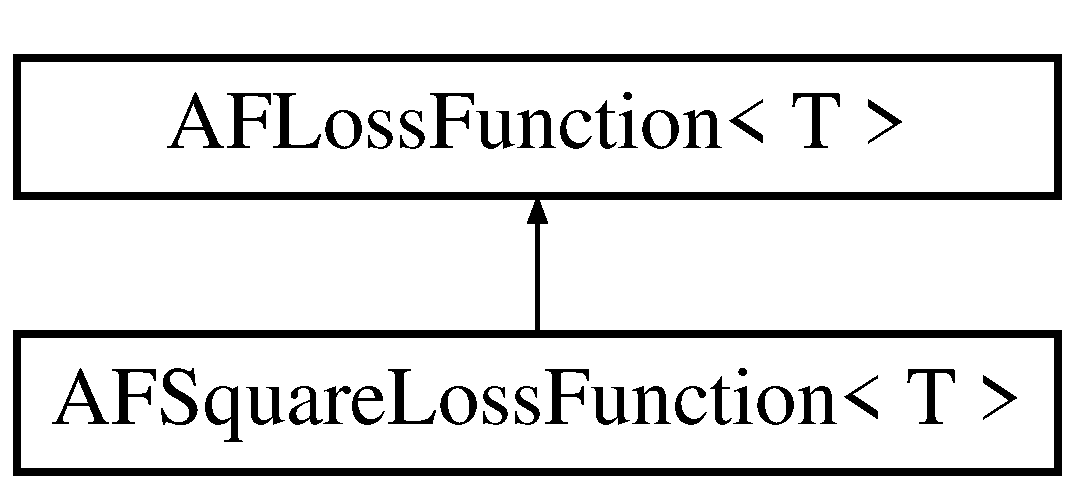
\includegraphics[height=2.000000cm]{classAFSquareLossFunction}
\end{center}
\end{figure}
\subsection*{Public Member Functions}
\begin{DoxyCompactItemize}
\item 
\mbox{\Hypertarget{classAFSquareLossFunction_a6bf89d61174eae853b603615a7e280a8}\label{classAFSquareLossFunction_a6bf89d61174eae853b603615a7e280a8}} 
T {\bfseries evaluate} (vector$<$ T $>$ $\ast$actual\+Vals, vector$<$ T $>$ $\ast$expected\+Vals)
\item 
void \hyperlink{classAFSquareLossFunction_abba069bd0b248fe89641673844b06616}{derivative} (vector$<$ T $>$ $\ast$actual\+Vals, vector$<$ T $>$ $\ast$expected\+Vals, vector$<$ T $>$ $\ast$output)
\end{DoxyCompactItemize}


\subsection{Member Function Documentation}
\mbox{\Hypertarget{classAFSquareLossFunction_abba069bd0b248fe89641673844b06616}\label{classAFSquareLossFunction_abba069bd0b248fe89641673844b06616}} 
\index{A\+F\+Square\+Loss\+Function@{A\+F\+Square\+Loss\+Function}!derivative@{derivative}}
\index{derivative@{derivative}!A\+F\+Square\+Loss\+Function@{A\+F\+Square\+Loss\+Function}}
\subsubsection{\texorpdfstring{derivative()}{derivative()}}
{\footnotesize\ttfamily template$<$typename T $>$ \\
void \hyperlink{classAFSquareLossFunction}{A\+F\+Square\+Loss\+Function}$<$ T $>$\+::derivative (\begin{DoxyParamCaption}\item[{vector$<$ T $>$ $\ast$}]{actual\+Vals,  }\item[{vector$<$ T $>$ $\ast$}]{expected\+Vals,  }\item[{vector$<$ T $>$ $\ast$}]{output }\end{DoxyParamCaption})\hspace{0.3cm}{\ttfamily [inline]}, {\ttfamily [virtual]}}

Finds derivative of squared loss L(input\+Val, actual\+Val, expected\+Val) w.\+r.\+t. actual\+Vals. 
\begin{DoxyParams}{Parameters}
{\em actual\+Vals} & \\
\hline
{\em expected\+Vals} & \\
\hline
{\em output} & \\
\hline
\end{DoxyParams}


Reimplemented from \hyperlink{classAFLossFunction}{A\+F\+Loss\+Function$<$ T $>$}.



The documentation for this class was generated from the following file\+:\begin{DoxyCompactItemize}
\item 
src/A\+F\+Functions.\+h\end{DoxyCompactItemize}

\hypertarget{classCrossEntropyLoss}{}\section{Cross\+Entropy\+Loss$<$ T $>$ Class Template Reference}
\label{classCrossEntropyLoss}\index{Cross\+Entropy\+Loss$<$ T $>$@{Cross\+Entropy\+Loss$<$ T $>$}}
Inheritance diagram for Cross\+Entropy\+Loss$<$ T $>$\+:\begin{figure}[H]
\begin{center}
\leavevmode
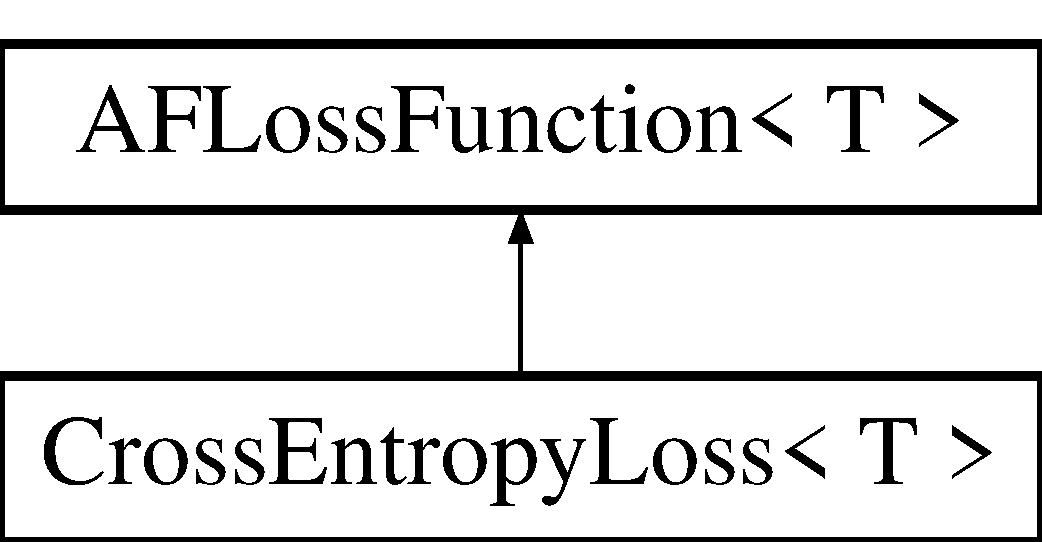
\includegraphics[height=2.000000cm]{classCrossEntropyLoss}
\end{center}
\end{figure}
\subsection*{Public Member Functions}
\begin{DoxyCompactItemize}
\item 
\mbox{\Hypertarget{classCrossEntropyLoss_a4ee9697f6272e7f94809e69ac85776d1}\label{classCrossEntropyLoss_a4ee9697f6272e7f94809e69ac85776d1}} 
T {\bfseries evaluate} (vector$<$ T $>$ $\ast$actual\+Vals, vector$<$ T $>$ $\ast$expected\+Vals)
\item 
void \hyperlink{classCrossEntropyLoss_a42d889334750f5a38e74dbce97b4a720}{derivative} (vector$<$ T $>$ $\ast$actual\+Vals, vector$<$ T $>$ $\ast$expected\+Vals, vector$<$ T $>$ $\ast$output)
\end{DoxyCompactItemize}


\subsection{Member Function Documentation}
\mbox{\Hypertarget{classCrossEntropyLoss_a42d889334750f5a38e74dbce97b4a720}\label{classCrossEntropyLoss_a42d889334750f5a38e74dbce97b4a720}} 
\index{Cross\+Entropy\+Loss@{Cross\+Entropy\+Loss}!derivative@{derivative}}
\index{derivative@{derivative}!Cross\+Entropy\+Loss@{Cross\+Entropy\+Loss}}
\subsubsection{\texorpdfstring{derivative()}{derivative()}}
{\footnotesize\ttfamily template$<$typename T $>$ \\
void \hyperlink{classCrossEntropyLoss}{Cross\+Entropy\+Loss}$<$ T $>$\+::derivative (\begin{DoxyParamCaption}\item[{vector$<$ T $>$ $\ast$}]{actual\+Vals,  }\item[{vector$<$ T $>$ $\ast$}]{expected\+Vals,  }\item[{vector$<$ T $>$ $\ast$}]{output }\end{DoxyParamCaption})\hspace{0.3cm}{\ttfamily [inline]}, {\ttfamily [virtual]}}

Finds derivative of squared loss L(input\+Val, actual\+Val, expected\+Val) w.\+r.\+t. actual\+Vals. 
\begin{DoxyParams}{Parameters}
{\em actual\+Vals} & \\
\hline
{\em expected\+Vals} & \\
\hline
{\em output} & \\
\hline
\end{DoxyParams}


Reimplemented from \hyperlink{classAFLossFunction}{A\+F\+Loss\+Function$<$ T $>$}.



The documentation for this class was generated from the following file\+:\begin{DoxyCompactItemize}
\item 
src/A\+F\+Functions.\+h\end{DoxyCompactItemize}

\hypertarget{classIdentityFunction}{}\section{Identity\+Function$<$ T $>$ Class Template Reference}
\label{classIdentityFunction}\index{Identity\+Function$<$ T $>$@{Identity\+Function$<$ T $>$}}
Inheritance diagram for Identity\+Function$<$ T $>$\+:\begin{figure}[H]
\begin{center}
\leavevmode
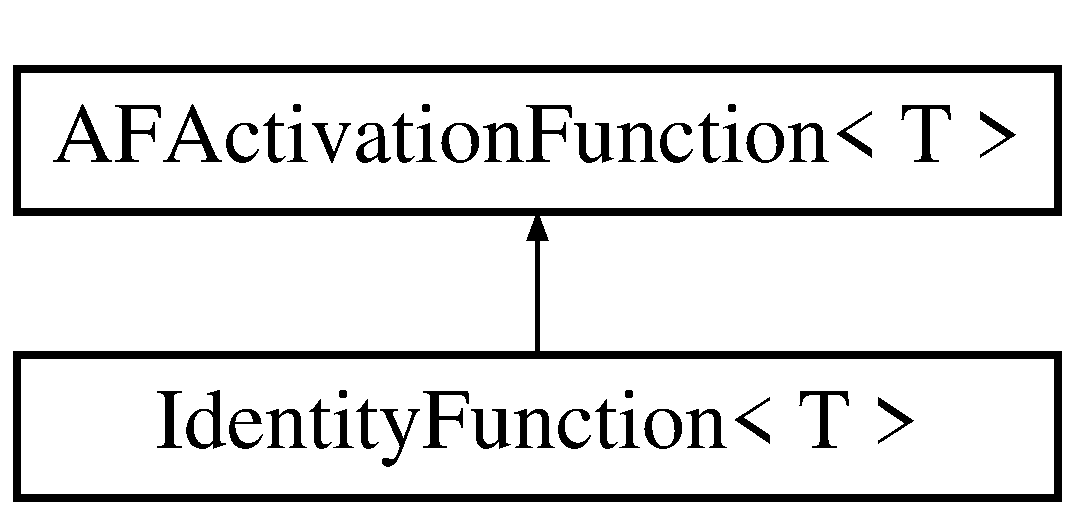
\includegraphics[height=2.000000cm]{classIdentityFunction}
\end{center}
\end{figure}
\subsection*{Public Member Functions}
\begin{DoxyCompactItemize}
\item 
\mbox{\Hypertarget{classIdentityFunction_a28558009eede686c44accf509bac0761}\label{classIdentityFunction_a28558009eede686c44accf509bac0761}} 
void {\bfseries evaluate} (vector$<$ T $>$ $\ast$input, vector$<$ T $>$ $\ast$output)
\item 
\mbox{\Hypertarget{classIdentityFunction_a62a12629a5cd78e7788d0a362e8d4b64}\label{classIdentityFunction_a62a12629a5cd78e7788d0a362e8d4b64}} 
void {\bfseries derivative} (vector$<$ T $>$ $\ast$input, vector$<$ T $>$ $\ast$output)
\end{DoxyCompactItemize}


The documentation for this class was generated from the following file\+:\begin{DoxyCompactItemize}
\item 
src/A\+F\+Functions.\+h\end{DoxyCompactItemize}

\hypertarget{classLayer}{}\section{Layer Class Reference}
\label{classLayer}\index{Layer@{Layer}}
\subsection*{Public Member Functions}
\begin{DoxyCompactItemize}
\item 
\hyperlink{classLayer_ac7b74e6fa9a90f78753c0318cf731719}{Layer} (size\+\_\+t \hyperlink{classLayer_a5f699c67410ebc5acad98cc5d3a9b5ec}{len\+In}, size\+\_\+t \hyperlink{classLayer_a57aa9a6491ea690f338f145c62a582f2}{len\+Out}, \hyperlink{classAFActivationFunction}{A\+F\+Activation\+Function}$<$ double $>$ $\ast$\hyperlink{classLayer_abe40a67ce33b17440ff6b0571b0c49e5}{activation\+Function})
\item 
\mbox{\Hypertarget{classLayer_ab725324396c041488c108238e0c23037}\label{classLayer_ab725324396c041488c108238e0c23037}} 
void {\bfseries randomize\+Weights} ()
\item 
void \hyperlink{classLayer_ad8fbfc2d20832ea5f8174074f26aaba1}{forward\+Pass} (vector$<$ double $>$ $\ast$\hyperlink{classLayer_ab72e6e0db19cd376c3c62b59e5f55e56}{input\+Vals}, vector$<$ double $>$ $\ast$\hyperlink{classLayer_a42731a44d761c086b0c4914fcc2ba8a0}{output\+Vals})
\item 
void \hyperlink{classLayer_ac447454d60f91693dc98020f0063da5a}{forward\+Pass} (vector$<$ double $>$ $\ast$\hyperlink{classLayer_ab72e6e0db19cd376c3c62b59e5f55e56}{input\+Vals})
\item 
void \hyperlink{classLayer_a5fa93a13d02fe9ee536d87b4980c8862}{backpropagate} (vector$<$ double $>$ $\ast$next\+Deltas, \hyperlink{classAFMatrix}{A\+F\+Matrix}$<$ double $>$ $\ast$next\+Weights, vector$<$ double $>$ $\ast$new\+Deltas)
\item 
void \hyperlink{classLayer_ab971a401b617ae20c5ab19310be25a70}{backpropagate} (vector$<$ double $>$ $\ast$next\+Deltas, \hyperlink{classAFMatrix}{A\+F\+Matrix}$<$ double $>$ $\ast$next\+Weights)
\item 
void \hyperlink{classLayer_a662f96aaa0e56564046baf34d4afddf5}{backpropagate\+Base} (vector$<$ double $>$ $\ast$actual\+Vals, vector$<$ double $>$ $\ast$expected\+Vals, \hyperlink{classAFLossFunction}{A\+F\+Loss\+Function}$<$ double $>$ $\ast$loss\+Fn, vector$<$ double $>$ $\ast$new\+Deltas)
\item 
void \hyperlink{classLayer_af2181f3eda8a8c6898d47fc3c280313b}{backpropagate\+Base} (vector$<$ double $>$ $\ast$actual\+Vals, vector$<$ double $>$ $\ast$expected\+Vals, \hyperlink{classAFLossFunction}{A\+F\+Loss\+Function}$<$ double $>$ $\ast$loss\+Fn)
\item 
\mbox{\Hypertarget{classLayer_a6896bb337eee9d535030fe115e4951ef}\label{classLayer_a6896bb337eee9d535030fe115e4951ef}} 
void {\bfseries update\+Weight\+Gradient} ()
\item 
\mbox{\Hypertarget{classLayer_a9617331c069ebe2a8f20fd72aa017717}\label{classLayer_a9617331c069ebe2a8f20fd72aa017717}} 
void {\bfseries update\+Weights} (double learning\+Rate)
\end{DoxyCompactItemize}
\subsection*{Public Attributes}
\begin{DoxyCompactItemize}
\item 
int \hyperlink{classLayer_a5f699c67410ebc5acad98cc5d3a9b5ec}{len\+In}
\begin{DoxyCompactList}\small\item\em The size of the vector that this layer takes as input. \end{DoxyCompactList}\item 
\mbox{\Hypertarget{classLayer_a57aa9a6491ea690f338f145c62a582f2}\label{classLayer_a57aa9a6491ea690f338f145c62a582f2}} 
int \hyperlink{classLayer_a57aa9a6491ea690f338f145c62a582f2}{len\+Out}
\begin{DoxyCompactList}\small\item\em The size of the vector that this layer outputs. \end{DoxyCompactList}\item 
\mbox{\Hypertarget{classLayer_ab72e6e0db19cd376c3c62b59e5f55e56}\label{classLayer_ab72e6e0db19cd376c3c62b59e5f55e56}} 
vector$<$ double $>$ $\ast$ \hyperlink{classLayer_ab72e6e0db19cd376c3c62b59e5f55e56}{input\+Vals}
\begin{DoxyCompactList}\small\item\em The values that this layer receives from the previous layer L\+E\+N\+\_\+\+IN. \end{DoxyCompactList}\item 
\mbox{\Hypertarget{classLayer_a615b17469874e0f1d9a63236568c1be4}\label{classLayer_a615b17469874e0f1d9a63236568c1be4}} 
vector$<$ double $>$ $\ast$ \hyperlink{classLayer_a615b17469874e0f1d9a63236568c1be4}{sums}
\begin{DoxyCompactList}\small\item\em The sums after the weights are multiplied by input value`. L\+E\+N\+\_\+\+O\+UT. \end{DoxyCompactList}\item 
\mbox{\Hypertarget{classLayer_a6ba44600aedf6e90536cd76dc94562c0}\label{classLayer_a6ba44600aedf6e90536cd76dc94562c0}} 
vector$<$ double $>$ $\ast$ \hyperlink{classLayer_a6ba44600aedf6e90536cd76dc94562c0}{deltas}
\begin{DoxyCompactList}\small\item\em The intermediate gradients of the loss, {\ttfamily deltas\mbox{[}i\mbox{]} = d(\+Error)/d(sum\+\_\+i)} L\+E\+N\+\_\+\+O\+UT. \end{DoxyCompactList}\item 
\mbox{\Hypertarget{classLayer_a42731a44d761c086b0c4914fcc2ba8a0}\label{classLayer_a42731a44d761c086b0c4914fcc2ba8a0}} 
vector$<$ double $>$ $\ast$ \hyperlink{classLayer_a42731a44d761c086b0c4914fcc2ba8a0}{output\+Vals}
\begin{DoxyCompactList}\small\item\em The values after the sums are put through the activation function. L\+E\+N\+\_\+\+O\+UT. \end{DoxyCompactList}\item 
\mbox{\Hypertarget{classLayer_acb311104d54fd7c09ea4c07006f8fc45}\label{classLayer_acb311104d54fd7c09ea4c07006f8fc45}} 
\hyperlink{classAFMatrix}{A\+F\+Matrix}$<$ double $>$ $\ast$ \hyperlink{classLayer_acb311104d54fd7c09ea4c07006f8fc45}{weights}
\begin{DoxyCompactList}\small\item\em The weights which are multiplied against the input values. This has {\ttfamily len\+Out} rows and {\ttfamily len\+In} cols. \end{DoxyCompactList}\item 
\mbox{\Hypertarget{classLayer_a8b36a2bc8a623ab02c0545097ebc967f}\label{classLayer_a8b36a2bc8a623ab02c0545097ebc967f}} 
\hyperlink{classAFMatrix}{A\+F\+Matrix}$<$ double $>$ $\ast$ \hyperlink{classLayer_a8b36a2bc8a623ab02c0545097ebc967f}{weight\+Gradient}
\begin{DoxyCompactList}\small\item\em The weight gradients. {\ttfamily weight\+Gradient\mbox{[}i,j\mbox{]} = d(\+Error)/d(weights\mbox{[}i,j\mbox{]})}. Same shape as {\ttfamily weights}. \end{DoxyCompactList}\item 
\mbox{\Hypertarget{classLayer_abe40a67ce33b17440ff6b0571b0c49e5}\label{classLayer_abe40a67ce33b17440ff6b0571b0c49e5}} 
\hyperlink{classAFActivationFunction}{A\+F\+Activation\+Function}$<$ double $>$ $\ast$ \hyperlink{classLayer_abe40a67ce33b17440ff6b0571b0c49e5}{activation\+Function}
\begin{DoxyCompactList}\small\item\em The activation function {\ttfamily g} such that `output\+Values = g(weights $\ast$ Input\+Vals). Note that g takes a vector. \end{DoxyCompactList}\end{DoxyCompactItemize}


\subsection{Constructor \& Destructor Documentation}
\mbox{\Hypertarget{classLayer_ac7b74e6fa9a90f78753c0318cf731719}\label{classLayer_ac7b74e6fa9a90f78753c0318cf731719}} 
\index{Layer@{Layer}!Layer@{Layer}}
\index{Layer@{Layer}!Layer@{Layer}}
\subsubsection{\texorpdfstring{Layer()}{Layer()}}
{\footnotesize\ttfamily Layer\+::\+Layer (\begin{DoxyParamCaption}\item[{size\+\_\+t}]{len\+In,  }\item[{size\+\_\+t}]{len\+Out,  }\item[{\hyperlink{classAFActivationFunction}{A\+F\+Activation\+Function}$<$ double $>$ $\ast$}]{activation\+Function }\end{DoxyParamCaption})\hspace{0.3cm}{\ttfamily [inline]}}


\begin{DoxyParams}{Parameters}
{\em len\+In} & The input length of this layer \\
\hline
{\em len\+Out} & The output size of this layer \\
\hline
{\em activation\+Fn} & Pass an \hyperlink{classAFActivationFunction}{A\+F\+Activation\+Function} by value so this layer knows how to calculate output values. \\
\hline
\end{DoxyParams}


\subsection{Member Function Documentation}
\mbox{\Hypertarget{classLayer_a5fa93a13d02fe9ee536d87b4980c8862}\label{classLayer_a5fa93a13d02fe9ee536d87b4980c8862}} 
\index{Layer@{Layer}!backpropagate@{backpropagate}}
\index{backpropagate@{backpropagate}!Layer@{Layer}}
\subsubsection{\texorpdfstring{backpropagate()}{backpropagate()}\hspace{0.1cm}{\footnotesize\ttfamily [1/2]}}
{\footnotesize\ttfamily void Layer\+::backpropagate (\begin{DoxyParamCaption}\item[{vector$<$ double $>$ $\ast$}]{next\+Deltas,  }\item[{\hyperlink{classAFMatrix}{A\+F\+Matrix}$<$ double $>$ $\ast$}]{next\+Weights,  }\item[{vector$<$ double $>$ $\ast$}]{new\+Deltas }\end{DoxyParamCaption})\hspace{0.3cm}{\ttfamily [inline]}}

Performs backpropogation algorithm. Writes this layer\textquotesingle{}s new d(\+Err)/d(Sums) into {\ttfamily new\+Deltas}. 
\begin{DoxyTemplParams}{Template Parameters}
{\em L\+E\+N\+\_\+\+O\+U\+T\+\_\+\+N\+E\+XT} & The next layer\textquotesingle{}s output length \\
\hline
\end{DoxyTemplParams}

\begin{DoxyParams}{Parameters}
{\em next\+Deltas} & The next layer\textquotesingle{}s d(\+Err)/d(sums); \\
\hline
{\em next\+Weights} & \\
\hline
{\em new\+Deltas} & \\
\hline
\end{DoxyParams}
\mbox{\Hypertarget{classLayer_ab971a401b617ae20c5ab19310be25a70}\label{classLayer_ab971a401b617ae20c5ab19310be25a70}} 
\index{Layer@{Layer}!backpropagate@{backpropagate}}
\index{backpropagate@{backpropagate}!Layer@{Layer}}
\subsubsection{\texorpdfstring{backpropagate()}{backpropagate()}\hspace{0.1cm}{\footnotesize\ttfamily [2/2]}}
{\footnotesize\ttfamily void Layer\+::backpropagate (\begin{DoxyParamCaption}\item[{vector$<$ double $>$ $\ast$}]{next\+Deltas,  }\item[{\hyperlink{classAFMatrix}{A\+F\+Matrix}$<$ double $>$ $\ast$}]{next\+Weights }\end{DoxyParamCaption})\hspace{0.3cm}{\ttfamily [inline]}}

Performs backpropogation algorithm and writes output to {\ttfamily this-\/$>$deltas}. 
\begin{DoxyTemplParams}{Template Parameters}
{\em L\+E\+N\+\_\+\+O\+U\+T\+\_\+\+N\+E\+XT} & \\
\hline
\end{DoxyTemplParams}

\begin{DoxyParams}{Parameters}
{\em next\+Deltas} & \\
\hline
{\em next\+Weights} & \\
\hline
\end{DoxyParams}
\mbox{\Hypertarget{classLayer_a662f96aaa0e56564046baf34d4afddf5}\label{classLayer_a662f96aaa0e56564046baf34d4afddf5}} 
\index{Layer@{Layer}!backpropagate\+Base@{backpropagate\+Base}}
\index{backpropagate\+Base@{backpropagate\+Base}!Layer@{Layer}}
\subsubsection{\texorpdfstring{backpropagate\+Base()}{backpropagateBase()}\hspace{0.1cm}{\footnotesize\ttfamily [1/2]}}
{\footnotesize\ttfamily void Layer\+::backpropagate\+Base (\begin{DoxyParamCaption}\item[{vector$<$ double $>$ $\ast$}]{actual\+Vals,  }\item[{vector$<$ double $>$ $\ast$}]{expected\+Vals,  }\item[{\hyperlink{classAFLossFunction}{A\+F\+Loss\+Function}$<$ double $>$ $\ast$}]{loss\+Fn,  }\item[{vector$<$ double $>$ $\ast$}]{new\+Deltas }\end{DoxyParamCaption})\hspace{0.3cm}{\ttfamily [inline]}}

The backprop algorithm for the last layer. First calculates {\ttfamily d(\+Err)/d(output\+Vals)}, which is the derivative of the loss function w.\+r.\+t to {\ttfamily actual\+Vals}. It then calculates d(\+Err)/d(sums)`.


\begin{DoxyParams}{Parameters}
{\em actual\+Vals} & \\
\hline
{\em expected\+Vals} & \\
\hline
{\em new\+Deltas} & \\
\hline
\end{DoxyParams}
\mbox{\Hypertarget{classLayer_af2181f3eda8a8c6898d47fc3c280313b}\label{classLayer_af2181f3eda8a8c6898d47fc3c280313b}} 
\index{Layer@{Layer}!backpropagate\+Base@{backpropagate\+Base}}
\index{backpropagate\+Base@{backpropagate\+Base}!Layer@{Layer}}
\subsubsection{\texorpdfstring{backpropagate\+Base()}{backpropagateBase()}\hspace{0.1cm}{\footnotesize\ttfamily [2/2]}}
{\footnotesize\ttfamily void Layer\+::backpropagate\+Base (\begin{DoxyParamCaption}\item[{vector$<$ double $>$ $\ast$}]{actual\+Vals,  }\item[{vector$<$ double $>$ $\ast$}]{expected\+Vals,  }\item[{\hyperlink{classAFLossFunction}{A\+F\+Loss\+Function}$<$ double $>$ $\ast$}]{loss\+Fn }\end{DoxyParamCaption})\hspace{0.3cm}{\ttfamily [inline]}}

The backprop algorithm for the last layer. First calculates {\ttfamily d(\+Err)/d(output\+Vals)}, which is the derivative of the loss function w.\+r.\+t to {\ttfamily actual\+Vals}. It then calculates d(\+Err)/d(sums)`.


\begin{DoxyParams}{Parameters}
{\em actual\+Vals} & \\
\hline
{\em expected\+Vals} & \\
\hline
{\em new\+Deltas} & \\
\hline
\end{DoxyParams}
\mbox{\Hypertarget{classLayer_ad8fbfc2d20832ea5f8174074f26aaba1}\label{classLayer_ad8fbfc2d20832ea5f8174074f26aaba1}} 
\index{Layer@{Layer}!forward\+Pass@{forward\+Pass}}
\index{forward\+Pass@{forward\+Pass}!Layer@{Layer}}
\subsubsection{\texorpdfstring{forward\+Pass()}{forwardPass()}\hspace{0.1cm}{\footnotesize\ttfamily [1/2]}}
{\footnotesize\ttfamily void Layer\+::forward\+Pass (\begin{DoxyParamCaption}\item[{vector$<$ double $>$ $\ast$}]{input\+Vals,  }\item[{vector$<$ double $>$ $\ast$}]{output\+Vals }\end{DoxyParamCaption})\hspace{0.3cm}{\ttfamily [inline]}}

Will perform the forward pass on this \hyperlink{classLayer}{Layer}. Will take in {\ttfamily input\+Vals}, calculate weighted sums, and then pass that result to this layer\textquotesingle{}s activation function. The output will be written to {\ttfamily output\+Vals}. 
\begin{DoxyParams}{Parameters}
{\em input\+Vals} & \\
\hline
{\em output\+Vals} & -\/ output\+Vals\mbox{[}i\mbox{]} = this-\/$>$weights.\+row(i).inner\+Product(input\+Vals). \\
\hline
\end{DoxyParams}
\mbox{\Hypertarget{classLayer_ac447454d60f91693dc98020f0063da5a}\label{classLayer_ac447454d60f91693dc98020f0063da5a}} 
\index{Layer@{Layer}!forward\+Pass@{forward\+Pass}}
\index{forward\+Pass@{forward\+Pass}!Layer@{Layer}}
\subsubsection{\texorpdfstring{forward\+Pass()}{forwardPass()}\hspace{0.1cm}{\footnotesize\ttfamily [2/2]}}
{\footnotesize\ttfamily void Layer\+::forward\+Pass (\begin{DoxyParamCaption}\item[{vector$<$ double $>$ $\ast$}]{input\+Vals }\end{DoxyParamCaption})\hspace{0.3cm}{\ttfamily [inline]}}

Will perform the forward pass on this \hyperlink{classLayer}{Layer}. Will take in {\ttfamily input\+Vals}, calculate weighted sums, and then pass that result to this layer\textquotesingle{}s activation function. The output will be written to {\ttfamily output\+Vals}. 
\begin{DoxyParams}{Parameters}
{\em input\+Vals} & \\
\hline
{\em output\+Vals} & -\/ output\+Vals\mbox{[}i\mbox{]} = this-\/$>$weights.\+row(i).inner\+Product(input\+Vals). \\
\hline
\end{DoxyParams}


\subsection{Member Data Documentation}
\mbox{\Hypertarget{classLayer_a5f699c67410ebc5acad98cc5d3a9b5ec}\label{classLayer_a5f699c67410ebc5acad98cc5d3a9b5ec}} 
\index{Layer@{Layer}!len\+In@{len\+In}}
\index{len\+In@{len\+In}!Layer@{Layer}}
\subsubsection{\texorpdfstring{len\+In}{lenIn}}
{\footnotesize\ttfamily int Layer\+::len\+In}



The size of the vector that this layer takes as input. 

Hello! 

The documentation for this class was generated from the following file\+:\begin{DoxyCompactItemize}
\item 
src/Layer.\+h\end{DoxyCompactItemize}

\hypertarget{classLeakyReLU}{}\section{Leaky\+Re\+LU$<$ T $>$ Class Template Reference}
\label{classLeakyReLU}\index{Leaky\+Re\+L\+U$<$ T $>$@{Leaky\+Re\+L\+U$<$ T $>$}}
Inheritance diagram for Leaky\+Re\+LU$<$ T $>$\+:\begin{figure}[H]
\begin{center}
\leavevmode
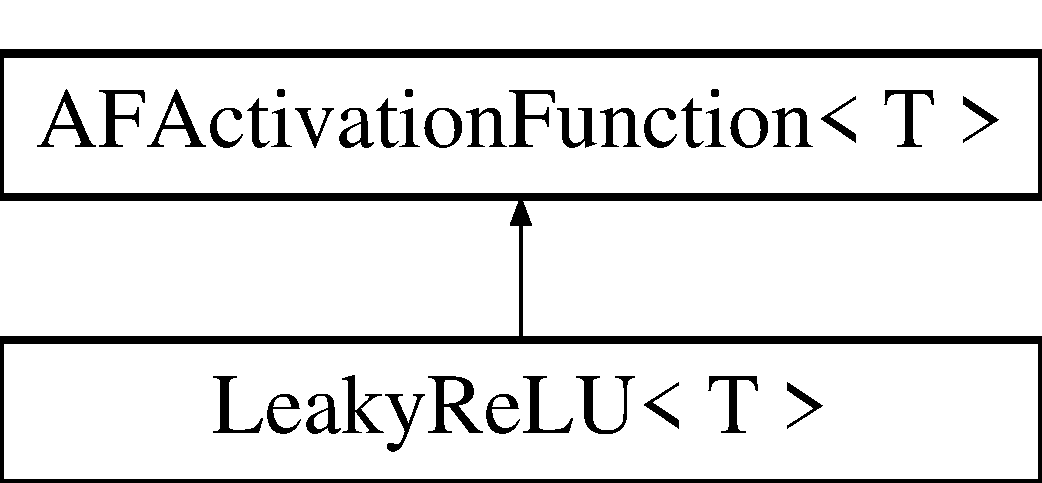
\includegraphics[height=2.000000cm]{classLeakyReLU}
\end{center}
\end{figure}
\subsection*{Public Member Functions}
\begin{DoxyCompactItemize}
\item 
\mbox{\Hypertarget{classLeakyReLU_ab4a3dab7ddb62df216333ab61dbdb0b9}\label{classLeakyReLU_ab4a3dab7ddb62df216333ab61dbdb0b9}} 
{\bfseries Leaky\+Re\+LU} (double leak\+Factor)
\item 
\mbox{\Hypertarget{classLeakyReLU_a9020ddae6a11791f60b253f6244016d3}\label{classLeakyReLU_a9020ddae6a11791f60b253f6244016d3}} 
void {\bfseries evaluate} (vector$<$ T $>$ $\ast$input, vector$<$ T $>$ $\ast$output)
\item 
\mbox{\Hypertarget{classLeakyReLU_ac85a6fb88ea4e3ea9d14bef0aa186298}\label{classLeakyReLU_ac85a6fb88ea4e3ea9d14bef0aa186298}} 
void {\bfseries derivative} (vector$<$ T $>$ $\ast$input, vector$<$ T $>$ $\ast$output)
\end{DoxyCompactItemize}
\subsection*{Public Attributes}
\begin{DoxyCompactItemize}
\item 
\mbox{\Hypertarget{classLeakyReLU_a7f9f45f3f44d69f4e7390e4b3b8d50a4}\label{classLeakyReLU_a7f9f45f3f44d69f4e7390e4b3b8d50a4}} 
double {\bfseries leak\+Factor}
\end{DoxyCompactItemize}


The documentation for this class was generated from the following file\+:\begin{DoxyCompactItemize}
\item 
src/A\+F\+Functions.\+h\end{DoxyCompactItemize}

\hypertarget{classLoader}{}\section{Loader Class Reference}
\label{classLoader}\index{Loader@{Loader}}
\subsection*{Public Member Functions}
\begin{DoxyCompactItemize}
\item 
\mbox{\Hypertarget{classLoader_a28f599170f85d5a6559e7d275bdfc471}\label{classLoader_a28f599170f85d5a6559e7d275bdfc471}} 
void {\bfseries load\+Xor\+Data} (vector$<$ vector$<$ double $>$$>$ $\ast$X, vector$<$ vector$<$ double $>$$>$ $\ast$Y)
\item 
\mbox{\Hypertarget{classLoader_ab9a9faa7ab6d4d2631fba357cc9e32d7}\label{classLoader_ab9a9faa7ab6d4d2631fba357cc9e32d7}} 
void {\bfseries load\+And\+Data} (vector$<$ vector$<$ double $>$$>$ $\ast$X, vector$<$ vector$<$ double $>$$>$ $\ast$Y)
\item 
\mbox{\Hypertarget{classLoader_a832154eb1851cfae11c522625a0c0e13}\label{classLoader_a832154eb1851cfae11c522625a0c0e13}} 
void {\bfseries load\+Or\+Data} (vector$<$ vector$<$ double $>$$>$ $\ast$X, vector$<$ vector$<$ double $>$$>$ $\ast$Y)
\item 
\mbox{\Hypertarget{classLoader_a6b4cf73255792a49420c8cb2d5db484a}\label{classLoader_a6b4cf73255792a49420c8cb2d5db484a}} 
void {\bfseries load\+Line\+Data} (vector$<$ vector$<$ double $>$$>$ $\ast$X, vector$<$ vector$<$ double $>$$>$ $\ast$Y, double slope, double intercept)
\end{DoxyCompactItemize}


The documentation for this class was generated from the following file\+:\begin{DoxyCompactItemize}
\item 
src/Loader.\+h\end{DoxyCompactItemize}

\hypertarget{classNet}{}\section{Net$<$ T $>$ Class Template Reference}
\label{classNet}\index{Net$<$ T $>$@{Net$<$ T $>$}}


{\ttfamily \#include $<$Net.\+h$>$}

\subsection*{Public Member Functions}
\begin{DoxyCompactItemize}
\item 
\mbox{\Hypertarget{classNet_a6885fd3c6502592b2ba34c84f69d28e2}\label{classNet_a6885fd3c6502592b2ba34c84f69d28e2}} 
{\bfseries Net} (vector$<$ \hyperlink{classLayer}{Layer} $\ast$$>$ $\ast$layers, \hyperlink{classAFLossFunction}{A\+F\+Loss\+Function}$<$ double $>$ $\ast$loss\+Function)
\item 
\mbox{\Hypertarget{classNet_a539b8a5584c3226381a5aeff1856a4d1}\label{classNet_a539b8a5584c3226381a5aeff1856a4d1}} 
double {\bfseries train\+Single} (vector$<$ T $>$ $\ast$input\+Vals, vector$<$ T $>$ $\ast$expected\+Vals)
\item 
\mbox{\Hypertarget{classNet_a26df53077f4d20578a10ad53b2d2a350}\label{classNet_a26df53077f4d20578a10ad53b2d2a350}} 
double {\bfseries train\+Epoch} (vector$<$ vector$<$ T $>$$>$ $\ast$all\+Input\+Vals, vector$<$ vector$<$ T $>$$>$ $\ast$all\+Expected\+Vals)
\item 
\mbox{\Hypertarget{classNet_ab2af642591b9445752a1359cdde3ac5b}\label{classNet_ab2af642591b9445752a1359cdde3ac5b}} 
double {\bfseries train} (vector$<$ vector$<$ T $>$$>$ $\ast$all\+Input\+Vals, vector$<$ vector$<$ T $>$$>$ $\ast$all\+Expected\+Vals, int num\+Epochs)
\end{DoxyCompactItemize}
\subsection*{Public Attributes}
\begin{DoxyCompactItemize}
\item 
\mbox{\Hypertarget{classNet_aa2ef9eb09a4ab5fe674365401639effd}\label{classNet_aa2ef9eb09a4ab5fe674365401639effd}} 
int {\bfseries num\+Layers}
\item 
\mbox{\Hypertarget{classNet_a915d9d7ce0ef4fb44961b22a11acce23}\label{classNet_a915d9d7ce0ef4fb44961b22a11acce23}} 
vector$<$ \hyperlink{classLayer}{Layer} $\ast$ $>$ $\ast$ {\bfseries layers}
\item 
\mbox{\Hypertarget{classNet_ab225fc71acaf5586f22d6f7b5cc7bd36}\label{classNet_ab225fc71acaf5586f22d6f7b5cc7bd36}} 
\hyperlink{classAFLossFunction}{A\+F\+Loss\+Function}$<$ double $>$ $\ast$ {\bfseries loss\+Fn}
\end{DoxyCompactItemize}


\subsection{Detailed Description}
\subsubsection*{template$<$typename T$>$\newline
class Net$<$ T $>$}

This is the \hyperlink{classNet}{Net} class documentation! This is a Plant\+U\+ML diagram of what happens  
\begin{DoxyTemplParams}{Template Parameters}
{\em T} & \\
\hline
\end{DoxyTemplParams}


The documentation for this class was generated from the following file\+:\begin{DoxyCompactItemize}
\item 
src/Net.\+h\end{DoxyCompactItemize}

\hypertarget{classReLU}{}\section{Re\+LU$<$ T $>$ Class Template Reference}
\label{classReLU}\index{Re\+L\+U$<$ T $>$@{Re\+L\+U$<$ T $>$}}
Inheritance diagram for Re\+LU$<$ T $>$\+:\begin{figure}[H]
\begin{center}
\leavevmode
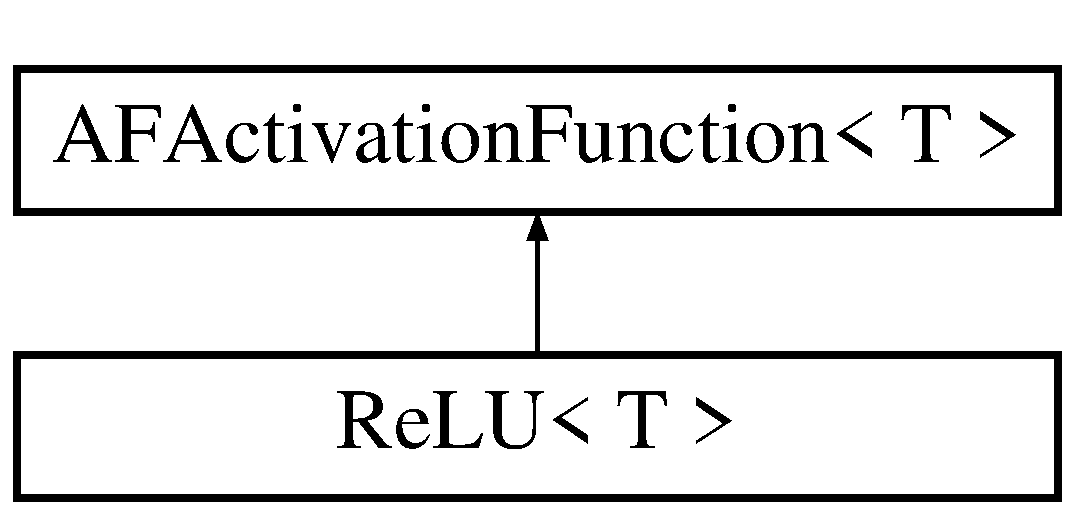
\includegraphics[height=2.000000cm]{classReLU}
\end{center}
\end{figure}
\subsection*{Public Member Functions}
\begin{DoxyCompactItemize}
\item 
\mbox{\Hypertarget{classReLU_adec5299ae40b276df20448ac26126bf9}\label{classReLU_adec5299ae40b276df20448ac26126bf9}} 
void {\bfseries evaluate} (vector$<$ T $>$ $\ast$input, vector$<$ T $>$ $\ast$output)
\item 
\mbox{\Hypertarget{classReLU_aeb172d142eb2806484e7765ad2bddc9a}\label{classReLU_aeb172d142eb2806484e7765ad2bddc9a}} 
void {\bfseries derivative} (vector$<$ T $>$ $\ast$input, vector$<$ T $>$ $\ast$output)
\end{DoxyCompactItemize}


The documentation for this class was generated from the following file\+:\begin{DoxyCompactItemize}
\item 
src/A\+F\+Functions.\+h\end{DoxyCompactItemize}

\hypertarget{classSoftmax}{}\section{Softmax$<$ T $>$ Class Template Reference}
\label{classSoftmax}\index{Softmax$<$ T $>$@{Softmax$<$ T $>$}}
Inheritance diagram for Softmax$<$ T $>$\+:\begin{figure}[H]
\begin{center}
\leavevmode
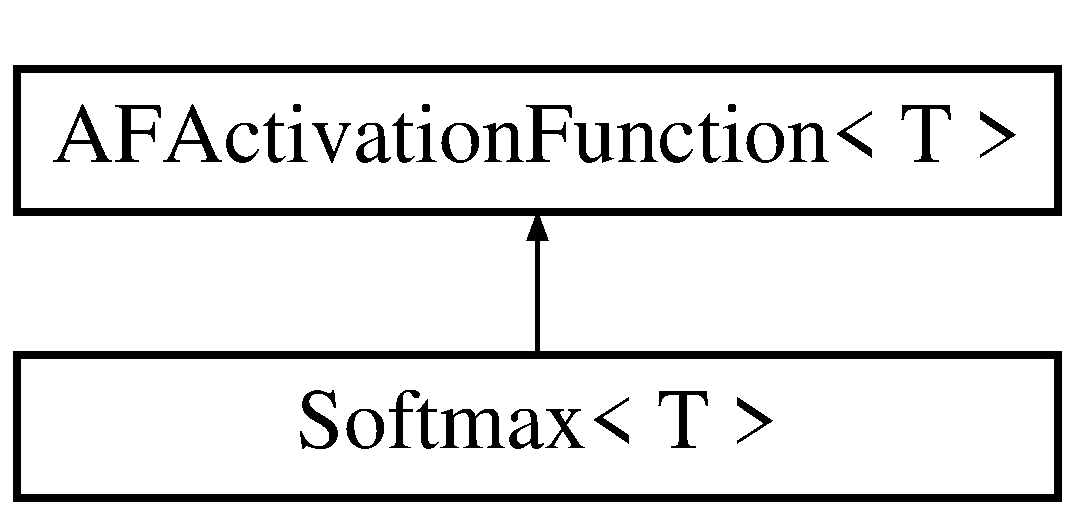
\includegraphics[height=2.000000cm]{classSoftmax}
\end{center}
\end{figure}
\subsection*{Public Member Functions}
\begin{DoxyCompactItemize}
\item 
\mbox{\Hypertarget{classSoftmax_a79fec04daf2c3fa8d234b0e1a0412b1e}\label{classSoftmax_a79fec04daf2c3fa8d234b0e1a0412b1e}} 
void {\bfseries evaluate} (vector$<$ T $>$ $\ast$input, vector$<$ T $>$ $\ast$output)
\item 
\mbox{\Hypertarget{classSoftmax_a2d61ce9b663c70c79bbac6e4b47d0c6d}\label{classSoftmax_a2d61ce9b663c70c79bbac6e4b47d0c6d}} 
void {\bfseries derivative} (vector$<$ T $>$ $\ast$input, vector$<$ T $>$ $\ast$output)
\end{DoxyCompactItemize}


The documentation for this class was generated from the following file\+:\begin{DoxyCompactItemize}
\item 
src/A\+F\+Functions.\+h\end{DoxyCompactItemize}

%--- End generated contents ---

% Index
\backmatter
\newpage
\phantomsection
\clearemptydoublepage
\addcontentsline{toc}{chapter}{Index}
\printindex

\end{document}
